\documentclass[conference,a4paper,12pt]{IEEEtran}
\IEEEoverridecommandlockouts

\usepackage{graphicx}
\begin{document}

\title{Report Homework Assignment 2: COP 6930 Special topics: Blockchain}

\author{\IEEEauthorblockN{Naman Arora}
\IEEEauthorblockA{\textit{UFID: 3979-0439} \\
\textit{University of Florida}\\
naman.arora@ufl.edu}
}

\maketitle

\begin{abstract}
This document is indented to serve as the report for completed homework assignment that it is attached with. The report goes through the justification of some of the choices made to complete the assignment, then through the procedure of running the code attached to extract results similar to the ones provided in expected output section at the end.
\end{abstract}

\section{Project Dependencies}
	\begin{itemize}
		\item{PostgreSQL:}
		The postgreSQL database is a very well respected and high preforming open source database query server. The kind of database provided for analysis was a good fit for conventional SQL based analysis.
		\item{Docker:}
		In the event of unavailability of the postgreSQL database server at hand, the repository is designed to run in dockerized container mode. A nice workflow is created with the help of helper scripts and is described in the next section.
		\item{sccs32s:}
		This project is leveraged to create a new addr\_sccs.dat file with joint+serial control.
	\end{itemize}


\section{Directory Structure}
	Since the repository is designed to run in both native and dockerized mode, there are a lot of helper scripts which demand explanation. After the explanation of the directory structure, both types of work flows will be introduced.

	\begin{figure}[h!]
	  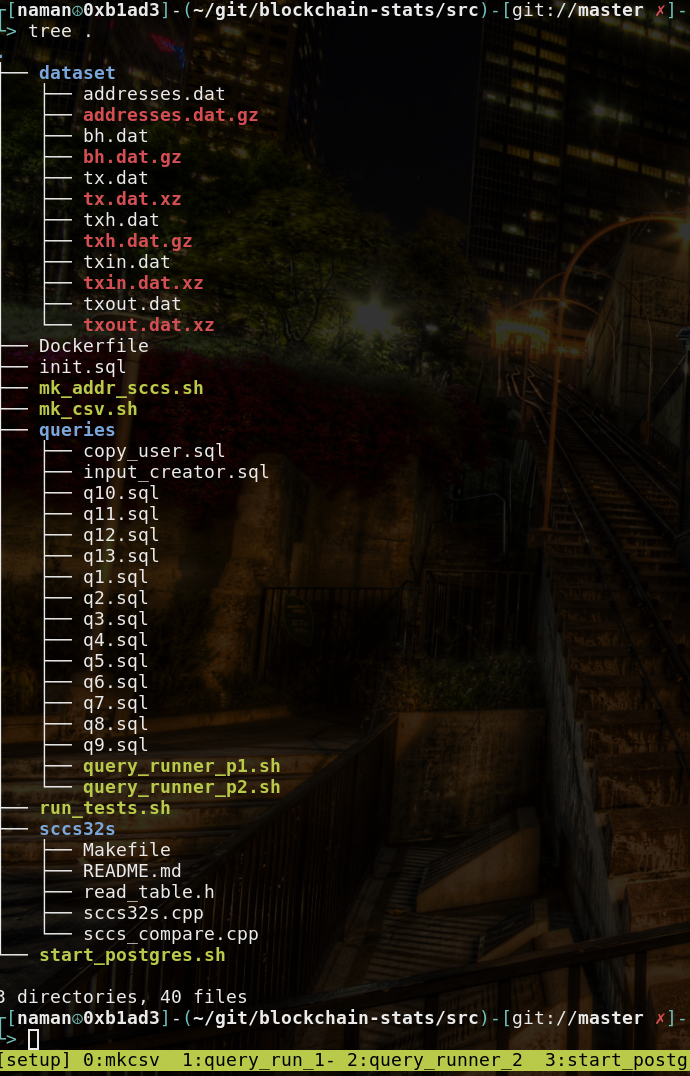
\includegraphics[width=\linewidth]{structure.png}
	  \caption{Directory Structure}
	  \label{Directory Structure}
	\end{figure}	
	
	\begin{itemize}
		\item{the src/dataset directory:}
		The project expects all the *.dat files to be present in this directory.
		\item{the src/queries direcotry:}
		This directory contains all the queries, one for every corresponding question in the assignment document along with two runner scripts, one for each part. All the query files have explanations within them in the form of comments.
		\item{The src/start\_postgres.sh script}
		This script starts up the postgres\_naman container. Before starting, though, it checks if docker is available, if the user running has permission to run docker and if such an image is available. In the last case, it builds the image from the provided Dockerfile and then runs it. In all the other cases, it fails.
		\item{The src/run\_tests.sh script:}
		This script assumes the container instance of postgresql\_naman image is up and running and ready to accept connections. It then runs all the queries in order, both part one and two, along with the formation of the addr\_sccs.dat file in between. All the outputs with their queries are printed on the stdout.
		\item{The src/mk\_addr\_sccs.sh script:}
		This helper script does as its name suggests, it requires that the dataset/out.csv file is present which is generated by the queries/input\_creator.sql query.
		
	\end{itemize}

\section{Instructions for running}
	\subsection{Dockerized workflow}
	Start the docker container
	
	\$ ./start\_postgresql.sh

	Run all the tests
		
	\$ ./run\_tests.sh
	
	
	\subsection{Native Workflow:}
	Assuming the postgresql is started, with all the tables created and default user as postgres,
	run the part 1
	
	\$ ./queries/query\_runner\_p1.sh queries
	
	Make the addr\_sccs.dat file
	
	\$./mk\_addr\_sccs.sh
	
	Run part2
	
	\$ ./queries/query\_runner\_p2.sh queries

	
\section{Output Screenshorts}

	\begin{figure}[h!]
	  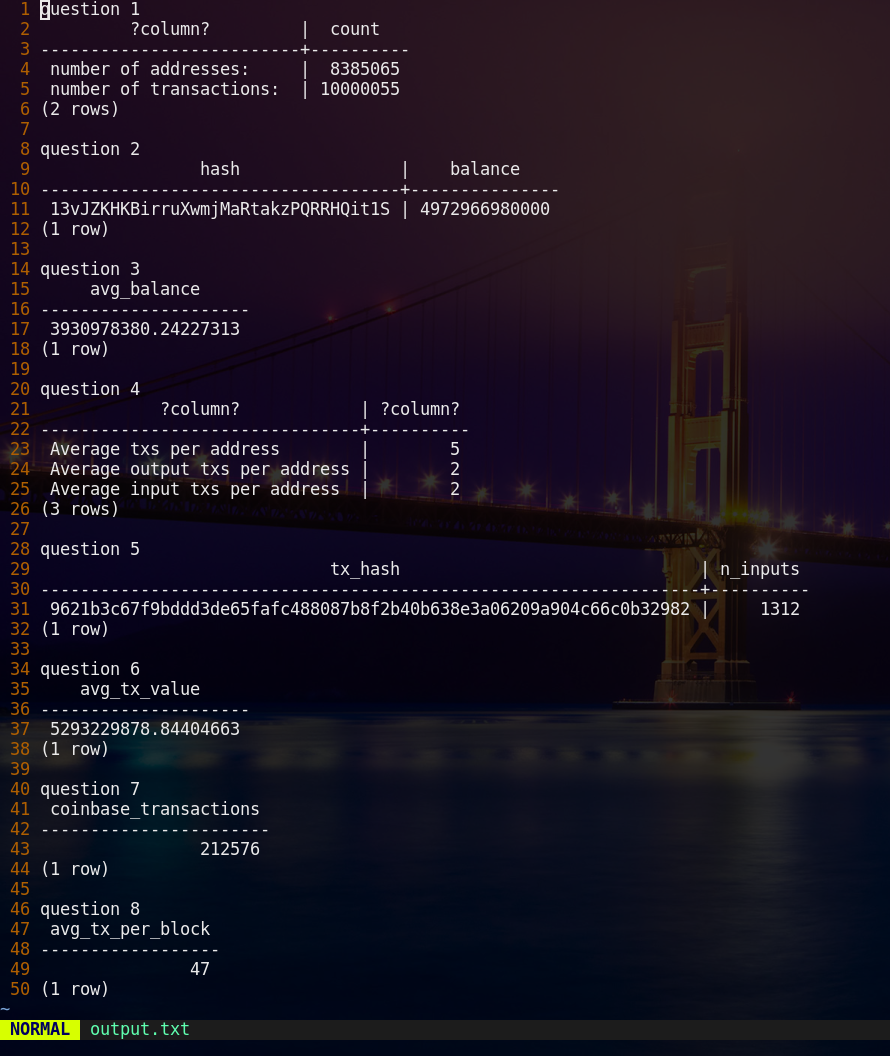
\includegraphics[width=\linewidth]{op1.png}
	  \caption{Output for Part 1}
	  \label{OP1}
	\end{figure}
	
	\begin{figure}[h!]
	  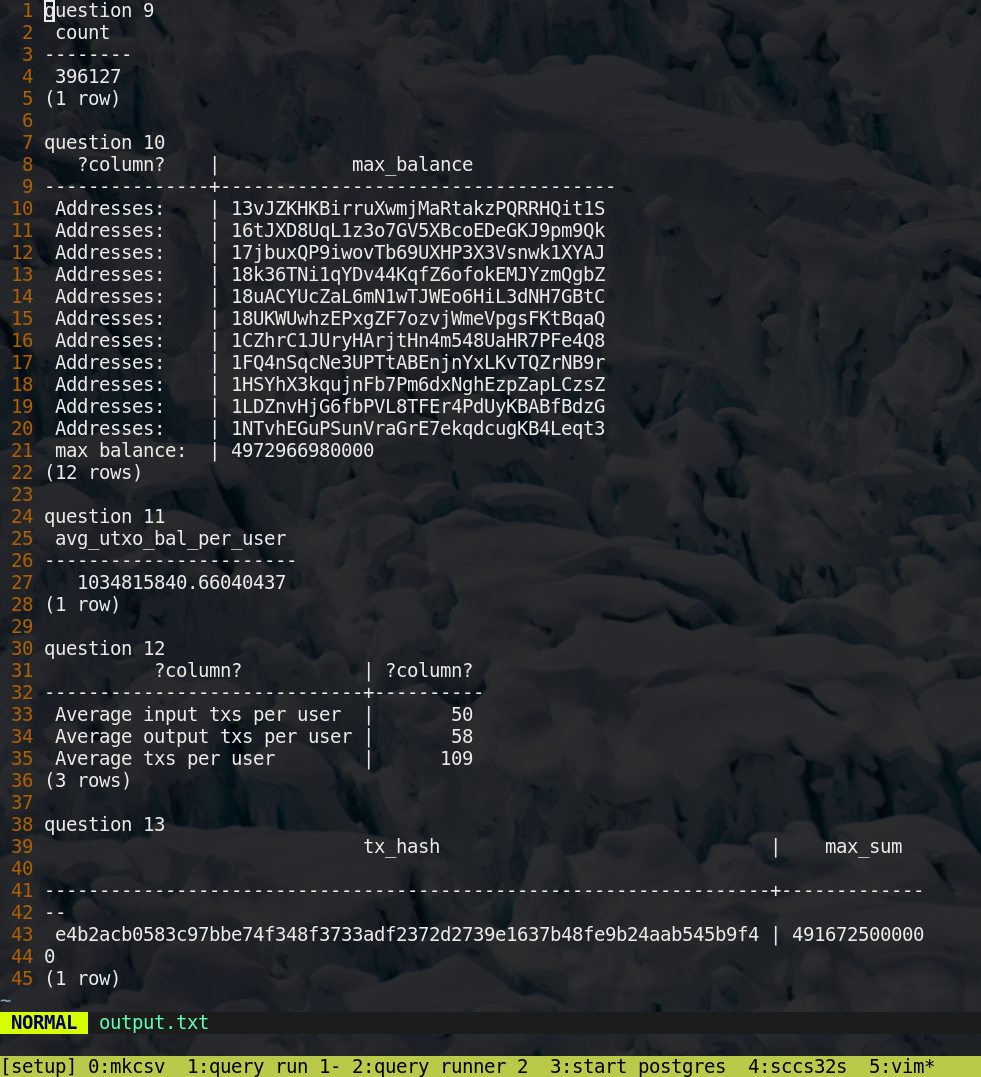
\includegraphics[width=\linewidth]{op2.png}
	  \caption{Output for Part 2}
	  \label{OP2}
	\end{figure}

\pagebreak

\section{Conclusion}
This concludes the homework assignment two. Even though considerable effort was made to write clever programs in C and parse the given database files, each effort tried to inevitably make a database implementation in some way or another. Hence, instead of reinventing the wheel, an established technology was used and effort was redirected to its deployment and execution. All the queries run a bit slower in the docker environment, taking up about 5-6 minutes in a hex core i7-8750H machine. Native workflow can easily make up for the time delay. All the code for the project is committed over at GitLab repository available at:

\begin{center}
https://gitlab.com/r0ck3r008/blockchain-stats
\end{center}

\end{document}